\documentclass{beamer}
\usepackage{pharmpresentation}
\usepackage{bbm}
\usepackage{amsmath}
\title{BlurNet: Defense by Filtering the Feature Maps}
\subtitle{Ravi Raju}

\begin{document}
\begin{frame}
	\titlepage
\end{frame}

\begin{frame}
\frametitle{Outline}
\tableofcontents
\end{frame}

\section{Introduction} % (fold)
\begin{frame}
\frametitle{Vulnerabilities in NNs}
\centering
\only<1> {
\includegraphics[scale=0.4]{clean_class1.png}\hspace{2.2cm}}
\only<2> {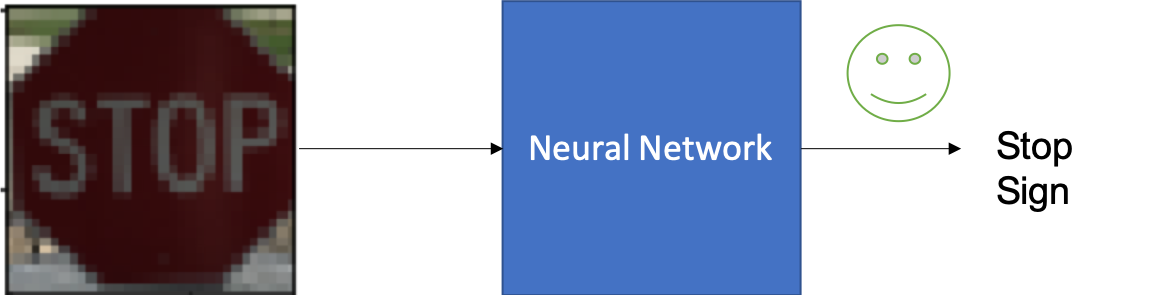
\includegraphics[scale=0.4]{cleanclassification2.png}}
\only<3> {
\includegraphics[scale=0.4]{advclassification1.png}\hspace{2.2cm}}
\only<4> {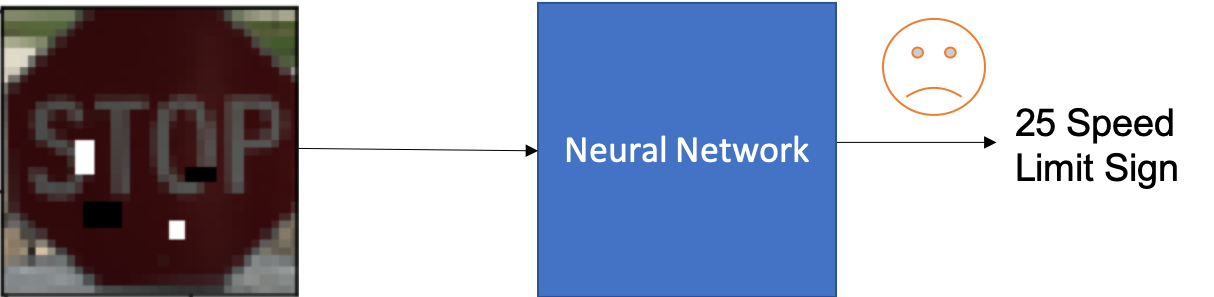
\includegraphics[scale=0.4]{advclassification2.png}}
\end{frame}

\begin{frame}
\frametitle{FFT Spectrum of Input Channels}
\begin{center}
	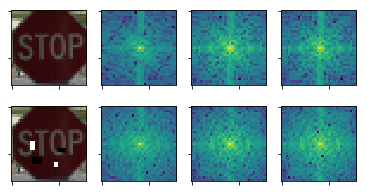
\includegraphics[scale=0.7]{regular_blur.png}
\end{center}
\begin{itemize}
	\item Log-shifted and normalized frequency spectrum of RGB channels of a natural and perturbed stop sign image
	\pause
	\item Lower freqencies correspond to the center and higher ones to the edge.  
\end{itemize}
\end{frame}

\begin{frame}
\frametitle{FFT of First Layer Feature Maps}
\begin{center}
	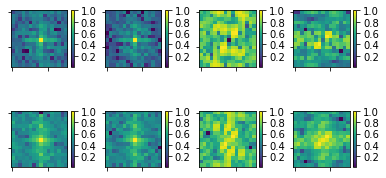
\includegraphics[scale=0.7]{fft_filters.png}
\end{center}
\begin{itemize}
	\item Each row corresponds to a unique feature map from L1 layer of network.
	\pause
	\item Difference image suggests that the perturbations induce high frequency components not found in natural stop signs
\end{itemize}
\end{frame}

\section{Background}

\begin{frame}{Terminology and Preliminaries: Adverserial Robustness}
	Let $x$ be an image and a neural network, $F(x) = y$, such that $F: \mathbb{R}^{h*w*c}\rightarrow \mathbb{R}$ where $y$ is the correct label.
	\begin{itemize}
		\item Main goal of an attacker - generating an image, $x_{adv}$ such that $F(x_{adv}) \neq y$ by perturbing the input pixels.
		\pause
		\item Main goal of a defense algorithm - classify the perturbed image with the correct label
		\pause
		\item Threat Model - rules which dictate what kind of information an attacker
		\begin{enumerate}
			\item White-box attacks - attacker has access to the model, architecture gradients, etc. \pause
			\item Black-box attacks (Transfer Attacks) - attacker has knowledge of model architecture but not parameters, etc.
		\end{enumerate}
	\end{itemize}
\end{frame}

\begin{frame}{Metrics}
	\begin{enumerate}
		\item Attack Success Rate - number of predictions altered by an attack, $\frac{1}{N}\sum_{n=1}^{N} \mathbbm{1}[F(x_n) \neq F(x_{nadv})]$.
		\pause
		\item $L_2$ Disimilarity Distance - how different is the adverserial image from the original, $\frac{1}{N}\sum^{N}_{n=1} \frac{||x - x_{adv}||_{p}}{||x_{adv}||_{p}}.$
		\pause
		\item An attacker is considered strong if its attack success rate is high while having a low dissimilarity metric.
	\end{enumerate}
\end{frame}

\begin{frame}{Attacker: Robust Physical Perturbation ($RP_2$) Attack}
	\centering
	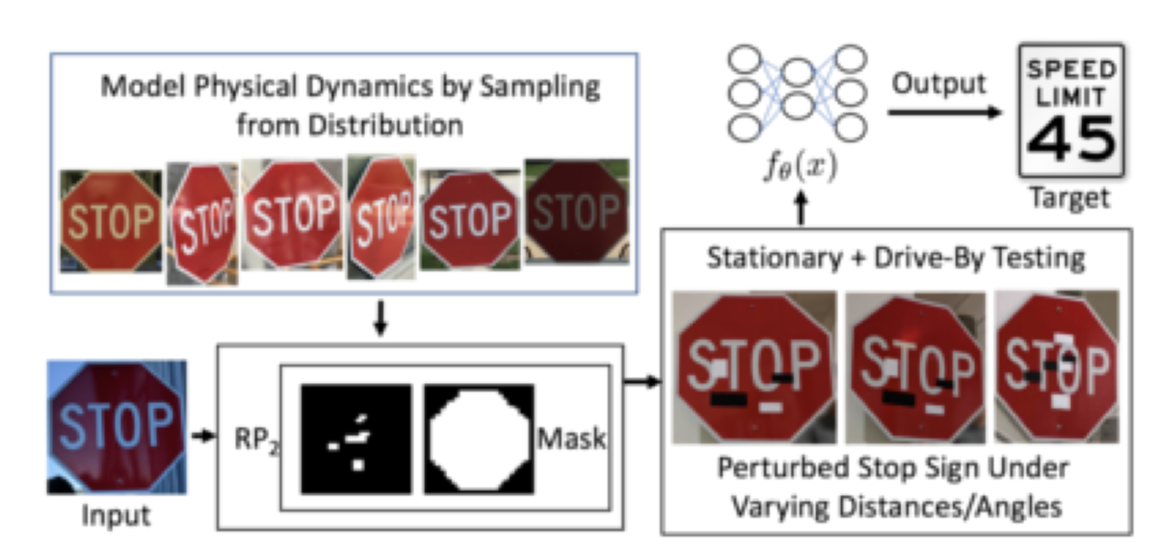
\includegraphics[scale=0.55]{RP2.png}
	\pause
	\begin{equation*}
	\arg \min_\delta \quad \lambda\lVert M_x \cdot \delta \rVert_p + \mathbb{E}_{x_i \sim X^V} J(f_\theta(x_i + T_i(M_x \cdot \delta)), y^*)
	\end{equation*}
\end{frame}

\section{Proposal}
\begin{frame}{Low-pass filtering}
	\centering
	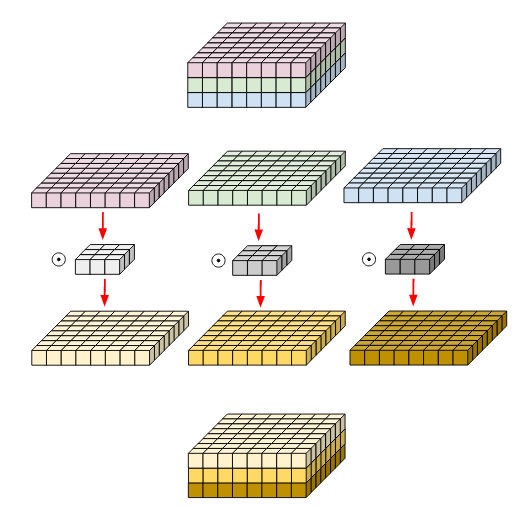
\includegraphics[scale=0.3]{depthwise_conv.png}
	\begin{itemize}
		\item Induce low-pass filtering with standard blur kernels by inserting a depthwise convolution after the first convolution layer.
	\end{itemize}
\end{frame}
\begin{frame}{Filtering input vs. Filtering Feature Maps}
\begin{table}[h!]
  \begin{center}
    \caption{Results from black box evaluation}
    \label{tab:transfer}
    \begin{tabular}{c|c|c} % <-- Alignments: 1st column left, 2nd middle and 3rd right, with vertical lines in between
      & \textbf{Accuracy} & \textbf{Attack Success Rate}\\
      \hline
      Baseline & 100\% & 90\%\\
      Input filter 3x3 & 100\% & 87.5\%\\
      Input filter 5x5 & 100\% & 67.5\%\\
      3x3 filter on L1 feature maps & 100\% & 65\%\\
      5x5 filter on L1 feature maps & 87.5\% & 17.5\%\\
    \end{tabular}
  \end{center}
\end{table}
\end{frame}

\begin{frame}{Filtering in the higher layers}
	\centering
	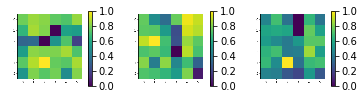
\includegraphics[scale=0.7]{higher_filters.png}
	\begin{enumerate}
		\item The FFT Spectrum of a subsampling of feature maps from the second layer of the network.
		\pause
		\item High frequency information is relevant to maintain decent classification.
	\end{enumerate}
\end{frame}

\section{Learning the Filter Parameters}
\begin{frame}{Minimizing accuracy loss}
	\centering
	\begin{itemize}
		\item Can we 
	\end{itemize}
\end{frame}
\begin{frame}{Whitebox Evaluation}
	\begin{table}[t!]
	  \begin{center}
	    \caption{Results from white box evaluation}
	    \label{tab:table2}
	    \scalebox{0.65}{\begin{tabular}{c|c|c|c|c|c} % <-- Alignments: 1st column left, 2nd middle and 3rd right, with vertical lines in between
	      & \textbf{$\alpha$} & \textbf{Legitimate Acc.} & \textbf{Average Success Rate} & \textbf{Worst Success Rate} & \textbf{$L_2$ Distortion}\\
	      \hline
	      Baseline & 0 & 91\% & 49.18\% & 90\% & 0.207\\
	      3x3 conv & $10^{-5}$ & 86.3\% & 30\% & 55\% & 0.201\\
	      5x5 conv & 0.1 & 86.3\% & 24.11\% & 47.5\% & 0.189\\
	      7x7 conv & 0.1 & 87\% & 11.61\% & 30\% & 0.203\\
	      TV & $10^{-4}$ & 85.6\% & 7.92\% & 17.5\% & 0.224\\
	      TV & $10^{-5}$ & 82.3\% & 8.47\% & 30\% & 0.199\\
	    \end{tabular}}
	  \end{center}
	\end{table}
\end{frame}


\begin{frame}{Whitebox Evaluation}
\begin{center}
	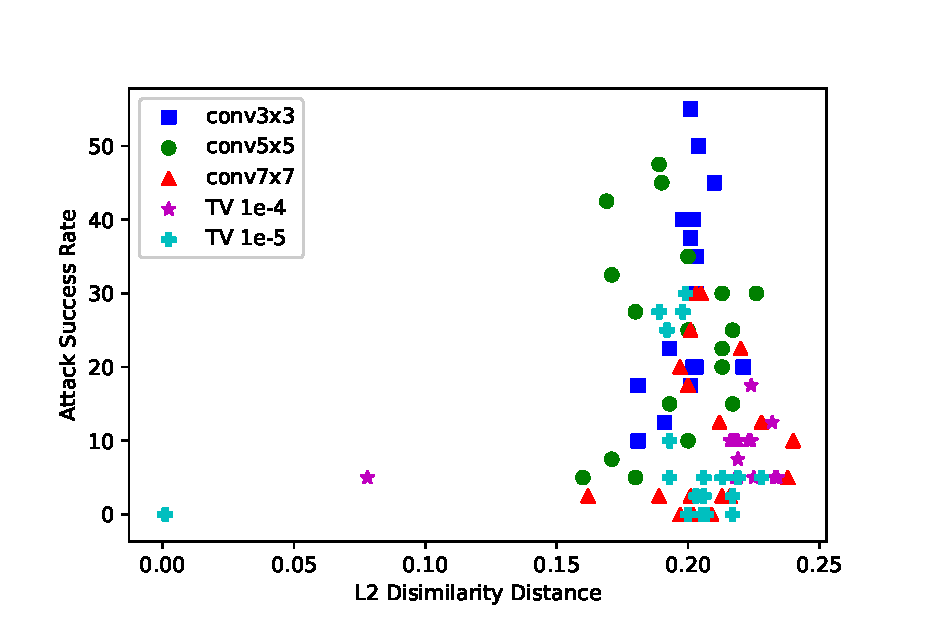
\includegraphics[scale=0.6]{L2vsAttkplot.eps}
\end{center}
\end{frame}

\end{document}